%%=============================================================================
%% Methodologie
%%=============================================================================

\chapter{\IfLanguageName{dutch}{Methodologie}{Methodology}}%
\label{ch:methodologie}

%% TODO: In dit hoofstuk geef je een korte toelichting over hoe je te werk bent
%% gegaan. Verdeel je onderzoek in grote fasen, en licht in elke fase toe wat
%% de doelstelling was, welke deliverables daar uit gekomen zijn, en welke
%% onderzoeksmethoden je daarbij toegepast hebt. Verantwoord waarom je
%% op deze manier te werk gegaan bent.
%%
%% Voorbeelden van zulke fasen zijn: literatuurstudie, opstellen van een
%% requirements-analyse, opstellen long-list (bij vergelijkende studie),
%% selectie van geschikte tools (bij vergelijkende studie, "short-list"),
%% opzetten testopstelling/PoC, uitvoeren testen en verzamelen
%% van resultaten, analyse van resultaten, ...
%%
%% !!!!! LET OP !!!!!
%%
%% Het is uitdrukkelijk NIET de bedoeling dat je het grootste deel van de corpus
%% van je bachelorproef in dit hoofstuk verwerkt! Dit hoofdstuk is eerder een
%% kort overzicht van je plan van aanpak.
%%
%% Maak voor elke fase (behalve het literatuuronderzoek) een NIEUW HOOFDSTUK aan
%% en geef het een gepaste titel.

This section contains a brief description of the road map to build the proof of concept (PoC), which combines the general key insights from the literature.

The proposed model can be seen as a three-way modular setup. Each step can be improved individually in order to acquire the best possible result and is implemented independently.
The first step focuses on localizing the athletes in the field in order to crop them out and spare computational resources. Next up is segmenting each skill performed in a given routine. The final part involves recognizing each isolated skill.

% TODO : chart overview of model.

\section{Jumper localization}

Jumper localization is needed in order crop a zoomed-in video of the skippers performing their routine. The AI generated image \ref{fig:sr2-performance-ai-generated} perfectly illustrates a competition setting, where the majority of the image and computation is lost on surroundings, judges and spectators.

For predicting the location of the athletes, any object detection model is fine with slight preference towards a model like YOLO or EfficientDet having a higher FPS rate than others based on survey of \textcite{Zaidi_2021}.
Using the predicted locations of the skippers, each frame of video can be cropped around the athletes.

Potential obstacles are predicted spectators or blurry athletes mid-skill being unrecognizable. Refer to the result chapter~\ref{ch:results} for more details on the solution.

\begin{figure}
    \centering
    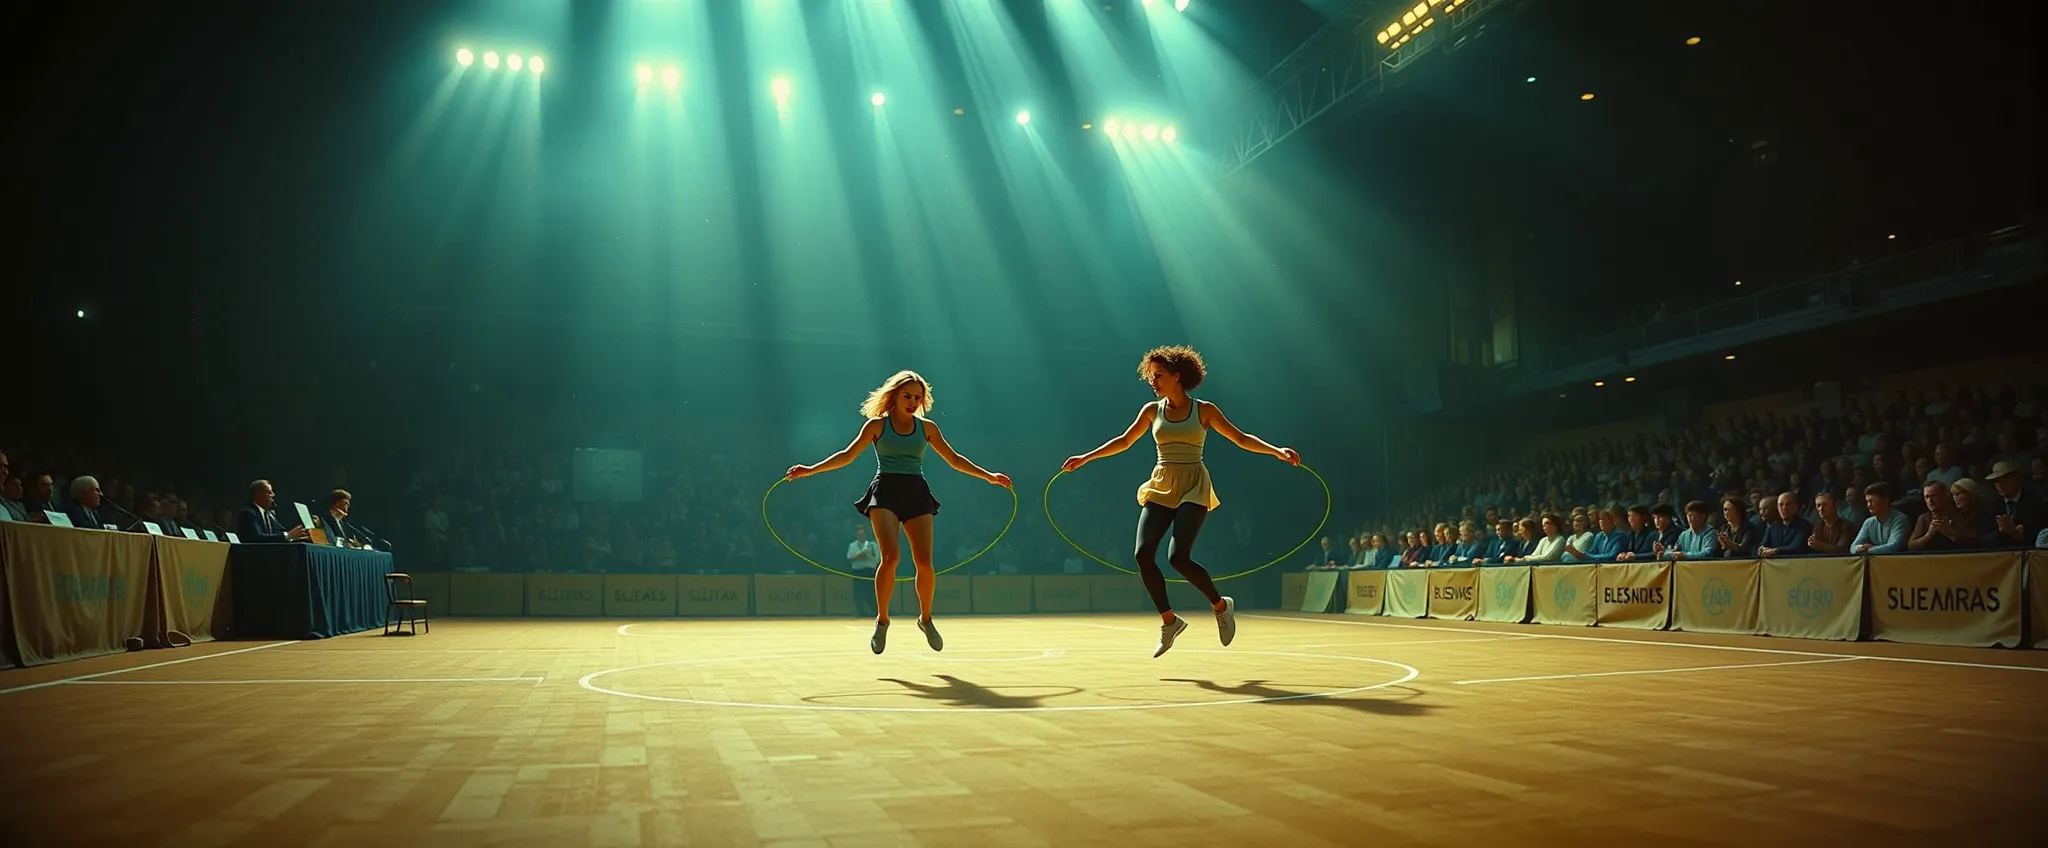
\includegraphics[width=0.95\linewidth]{img/sr2-performance-ai-generated-HF-cinedifusion.png}
    \caption[AI Generated image using takajordans CineDiffusion implementation on huggingface of two skippers performing a single rope 2 freestyle in front of judges and public]{AI Generated image using takajordans CineDiffusion implementation on huggingface of two skippers performing a single rope 2 freestyle in front of judges and public \autocite{HF_takarajordan_CineDiffusion}.}
    \label{fig:sr2-performance-ai-generated}
\end{figure}


\section{Action segmentation}

The main purpose of the action segmentation is to enable predictions on full routines in order to actually use the whole model. Using the cropped images, and the assigned start and end frame of a skill, the model can predict whether a given frame is an interesting split point or not.

For jump rope, this mostly means moments when an athlete leaves or lands on the floor. However there are special cases such as cartwheels. Only moments when either hands or feet landed over a rope, then only ends the skill. A couple of models can be tried as the idea of leaving and landing on the floor seems relatively straightforward. This means more simple convolutional models to models incorporating temporal information.
The best model or an ensemble of the best ones will be used in the full sequence.

A couple of ideas exist in order mark interesting split moments. Both the frame before and the frame after each split point can be assigned as split point, selecting the one with the highest probability as the final split point. Another idea would be to assign higher values to split points using a cyclic function like the sinus depending on its distance between two split points.

\section{Skill recognition}

The last part involves recognizing the performed skill, which is, as introduced in the literature, a combination of different aspects. What are the turners doing, using one or both arms, an additional body rotation, etc.
For this part, a video vision model is definitely required to fill in the temporal information, e.g. amount of rotations.
Along the way, additional aspects to a skill label can be added in order to incorporate every level and skill or once-in-a-lifetime skills can be marked as unknown in order for the model to be robust in predicting new skills. Each prediction can then be mapped to its corresponding level.
Multiple different models can be tried in order to find the best one.


\section{Model verification}

Finally, when skills are predictable, a comparison between the jury assigned scores, the models prediction and the effective score can be made in order to check whether model predictions could be used or more research/training is needed. This is an additional check, beside the accuracy of the model or confusion matrices.

